%# -*- coding: utf-8-unix -*-
%%==================================================
%% chapter02.tex
%%==================================================

%\bibliographystyle{sjtu2}%[此处用于每章都生产参考文献]
\chapter{WEB设计开发理论、技术和工具}
\label{chap:web_dev}
软件工程是研究和应用如何以系统性的、规范化的、可定量的过程化方法去开发和维护软件\supercite{radatz1990ieee},以及如何把经过时间考验而证明正确的管理技术和当前能够得到的最好的技术方法结合起来的学科。它涉及到程序设计语言、数据库、软件开发工具、系统平台、标准、设计模式等方面。所以本课题首先学习了软件开发尤其是WEB开发的相关理论,调研、比较并选择了一些主流的WEB开发技术和高效的WEB开发工具,以期能够用快速、高效、低成本地完成系统的开发。
\section{设计理论}
本系统在开发速度、可重用性、UI/UE、响应式、实时性等方面具有较高的要求,这就意味着传统的瀑布式开发、CSS+HTML、ajax请求等WEB开发理论不能达到本系统的要求。本章学习的理论可以给开发明确可行性、指明开发的方向、提高效率、减少重复造轮子,从而保证系统的顺利实现。
\subsection{敏捷开发}
敏捷开发有很多种,它们的具体名称、理念、过程、术语都不尽相同,相对于「非敏捷」,更强调程序员团队与业务专家之间的紧密协作、面对面的沟通(认为比书面的文档更有效)、频繁交付新的软件版本、紧凑而自我组织型的团队、能够很好地适应需求变化的代码编写和团队组织方法,也更注重软件开发過程中人的作用。\supercite{beck2013agile}

Clarity是一家创业公司,业务需求变化迅速,人员结构比较精简,因此更加适合用敏捷开发。本系统的软件开发团队由3个人组成,每天早晨与需求方即公司CEO和硬件开发团队进行视频通话来总结前一天的开发进度和确定当天的开发任务,不断地在测试服务器部署新特性(feature)版本和在生产服务器部署热修复(hotfix)版本,每个特性完成后再正式发布(release)到生产服务器上,团队成员吃住同行、分工灵活,每个人都能独当一面。
\subsection{Web Components}
Web Components是一组现在已经被W3C加入HTML和DOM规范的、为Web提供了一套标准组件模型的浏览器新特性,它们的设计理念是把“基于组件的软件工程”\footnote{软件工程的一个分支,是一种基于重用的定义、实现和组合松散的独立组件的软件来开发系统的方法}带到互联网的世界。Web Components主要包括4个特性:
\begin{description}
  \item[自定义元素(Custom Elements)] 定义新的HTML元素的应用程序接口
  \item[影DOM(Shadow DOM)] 兼具封装性和可组合性的DOM和样式
  \item[HTML 引入(HTML Imports)] 可声明的引入HTML文档到其他HTML文档的方法
  \item[HTML 模板(HTML Templates)] 新的<template>\footnote{\url{https://developer.mozilla.org/en-US/docs/Web/HTML/Element/template}}标签,允许HTML文档包含惰性(延后定义或加载)的DOM块
\end{description}

本系统的软件开发团队接受过良好的软件工程教育,对于重复造轮子这样的事情是坚决抵制的,所以我们对于组件的可重用性要求非常高。虽然本系统最终没有直接使用Web Components的官方实现Polymer,但其中自定义元素、HTML 引入和HTML 模板等特性都是非常有意义的,本系统中使用的Angular和React都有这些理念的原型,本系统在实现组件时也大量使用了这些概念来做到组件的可重用性。

\subsection{Material-design}
Material Design,代号为Quantum Paper\footnote{\url{http://www.androidpolice.com/2014/06/11/exclusive-quantum-paper-and-googles-upcoming-effort-to-make-consistent-ui-simple/}}, 是由Google推出的一种全新的设计语言,旨在为手机、平板、台式机等不同平台提供更加一致且广泛的外观和感觉。Material Design 总体来讲是一种隐喻式的基于纸张和墨水的设计,元素是扁平的、有阴影的,按照各自的高度浮动在背景上方,接缝和阴影让你知道哪些元素是可以触碰到的(操作的)。当你移动或改变它们的高度的时候,感觉是一张纸在被移动,符合人们对三维物体的直觉,与真实的纸不同之处在于Material Design的纸可以智能的伸缩和变形。

Clarity的CEO本人是一名正在读本科的大学生,从创业伊始就对不管是硬件还是软件要求都特别高,在UI方面尤其如此,Material Design是为数不多的能满足他的要求的设计语言。本系统中版本管理模块和Smart City模块都使用了Material Design,深受设计师、程序员和用户喜爱,因为在这套设计语言的基础上,设计师省去了很多繁琐的顾虑,程序员实现时也有比较好的UI库,界面简洁明了,让用户直观地感受到页面上不同层次不同元素的重要性。

\subsection{响应式设计 和 Flex 布局}
响应式设计是一种WEB设计方法,旨在构建出可以提供跨设备的(从桌面电脑到移动设备)拥有最佳的视觉和交互体验的网站,方便用户使用最少的缩放、平移和滚动操作来阅读和浏览。\supercite{marcotte2013responsive}为自动适应浏览者的设备环境,响应式网站使用流式的基于比例的网格布局,弹性的图片和CC3 media queries\footnote{没有正式的中文译名,直译为媒体查询,是CSS中@media规则的扩展}做到了以下几点:
\begin{description}
  \item[流式网格] 流式网格要求页面元素按照如百分比之类的相对单位来缩放而不是传统的如像素或点的绝对单位;
  \item[弹性图片] 为防止图片显示时超出容器范围,弹性图片也按照相对单位来缩放;
  \item[Media queries] Media queries 允许页面上的元素根据显示设备的某种属性来使用不同的样式,这里的属性主要是设备的宽度;
\end{description}

Flex 布局,全称CSS Flex Box Layout,意思为弹性盒状模型布局,它是由W3C在2009年提出的一种新的布局方案,可以简便地、完整地、响应式地实现各种简单或复杂的页面布局,目前所有主流浏览器都支持Flex 布局。

Clarity作为一家创业公司没有那么多精力同时维护不同平台上的应用,因此虽然目前并不要求适配手机,但起码的屏幕宽度兼容是需要的,为将来适配更小的屏幕打好基础。本系统中三个模块都使用了flex布局,从而使得页面上的元素可以随着设备屏幕大小的变化(或浏览器的缩放)而自动伸缩。虽然我们的系统不需要适配手机,但其中版本管理模块因为页面上有比较宽的列表,在窄屏幕上显示不正常,于是采用了响应式设计来避免这个问题。
\subsection{RESTful API设计和Web Socket数据更新}
RESTful 中文名叫“具象状态传输”,全称“Representational state transfer”,它是一种包含一系列同在一个分布式网络系统中协调的组件、连接器和数据元素如何按照不同的角色进行交互的设计原则(或者叫设计风格),旨在促进系统的性能、可扩展性、简单性、可修改性、可读性、便携性和可靠性。\supercite{fielding2002principled,fielding2000architectural}相比于SOAP\footnote{Simple Object Access protocol,简单对象访问协议}和XML-RPC\footnote{XML(标准通用标记语言下的一个子集)远程方法调用}更加简单轻量,在URL处理和Payload编码上更加简洁明了。这套设计原则并不局限于WEB应用程序,只要满足其约束条件的和原则的应用程序或设计就是RESTful。WEB应用程序最重要的REST原则是,客户端和服务器之间的交互在不同请求之间是无状态的,这就意味着服务器可以随时重启并且客户端并不关心连接的是哪台服务器,这十分适合云计算\footnote{提供动态的易扩展的虚拟化计算资源的互联网服务模式}的环境。

WebSocket 是HTML5\footnote{万维网的核心语言、标准通用标记语言下的一个应用超文本标记语言(HTML)的第五次重大修改}中一种新的通信协议,浏览器与服务器通过一个TCP\footnote{即Transmission Control Protocol 传输控制协议}连接上的全双工通信(full-duplex)进行交互,只有一开始的握手需要借助HTTP\footnote{即HyperText Transfer Protocol超文本传输协议,是互联网上应用最为广泛的一种网络协议}请求完成。它使得浏览器可以和网站进行更多更频繁更实时的交互,从而可以摒弃从前通过轮询\footnote{每隔一秒向服务器发送一个HTTP请求来获取最新数据}来获取最新数据却会给服务器带来沉重负担的方法。

Clarity如其他众多创业公司一样,选择使用云服务器来搭载自己的服务,因为其自动扩展的虚拟化资源无论是直接成本还是管理成本都比自己公司搭建服务器低。本系统搭载在AWS云服务器上,无状态交互是可扩展性的一大保障,频繁地增删改查设备等数据资源也需要RESTful,于是设计了一套RESTful风格的API,前端和后端分别遵循API接口来实现。另一方面需要让用户能够实时地看到自己的修改以及空气质量的变化,本系统使用WebSocket来实时地更新数据,前后端分别使用收听和发送相关主题(topic)。
\subsection{Oauth 和 JWT}
OAuth是Open Authorization的简写,它是一个被广泛用作互联网用户使用它们的微软、Google、Facebook、Twitter等账号在不用输入它们的密码的情况下登录到第三方网站的开放授权标准。一般来讲,OAuth提供给客户端一个代表资源拥有者访问服务器资源的“安全访问授权”。它规定了资源拥有者授权第三方访问其服务器资源而无需共享它们的凭据的过程。它是专门为超文本传输协议(HTTP)设计的,本质上OAuth允许一个授权服务器在资源拥有者批准的情况下直接把访问令牌(Access Token)发送到第三方客户端,然后第三方再使用访问令牌来获取资源服务器上被保护的资源。\supercite{hardt4rfc6749}

JWT 是 JSON Web Token的简写,它是一个用来在WEB应用环境下在不同参与者之间传递声明(claims)的开放标准。这些令牌被巧妙地设计成紧凑、URL安全且可用的,最适合使用在浏览器单点登录\footnote{SSO, single sign-on}的情况下。JWT声明被典型地用于在身份提供者和服务提供者或者任何其他业务过程中需要身份的地方之间传递认证用户的身份识别。\supercite{bradley2015json}这些令牌本身也可以被认证和加密。

Clarity虽然业务规模还不大,用户数量也很少,但在安全认证方面也是紧跟行业潮流,为将来接入各种社交账号登录做准备。本系统使用OAuth标准,其中访问令牌(Access Token)使用的是JWT。用户登陆后除了会获得一个对应的访问令牌之外还有一个寿命较长的刷新令牌(Refresh Token)用来在用户短期离线后自动刷新访问令牌,而这一切除了一开始的登录都不需要用户重新输入密码,只有在用户长期离线刷新令牌也过期的情况下才需要再次登录。

\subsection{Flux 架构模式}
Flux 是Facebook用来构建客户端WEB应用的应用架构,它利用一个单向的数据流对React\footnote{会在下一节技术架构中介绍到}的可组合的试图组建进行了有力的补充。它更像是一种模式而不是一个框架,所以在这里本课题认为它属于理论而不是技术。

它与传统的MVC模型\footnote{即Model View Controller,是一种软件设计典范}不同,主要包括三部分:dispatcher、store和view,由action来触发状态(state)变化。如下图所示: 所有的action会进入到dispatcher进行处理,dispatcher会产生新的state用以更新store,store选择恰当的时机更新后通过view提前注册好的消息(回调)来告诉view更新用户界面。但其实大部分情况下action由用户的操作产生,因此会有从view产生的action。

\begin{figure}[!htp]
 \centering
 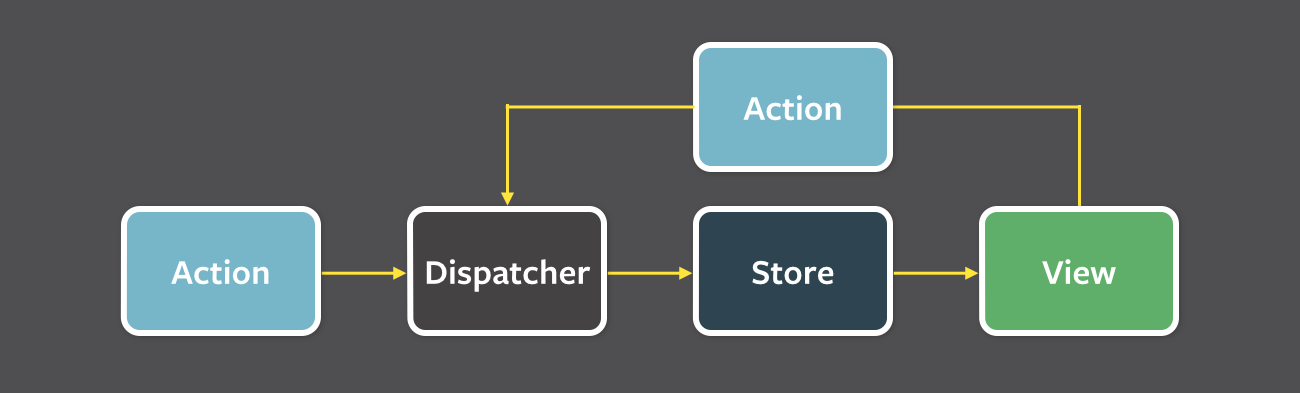
\includegraphics[width=0.9\textwidth]{flux.png}
 \bicaption[fig:longcaptionbad]{Flux 单向数据流}{Flux 单向数据流}{Fig}{Flux Unidirectional Data Flow}
\end{figure}

单向数据流传输的Flux不会像MVC那样,一旦系统复杂了,model和view之间的联系呈几何级数增长,也不会像双向绑定那样,一旦绑定层数多了,连程序员自己都不清楚状态更新是被哪里触发的。

Clarity致力于给用户最好的体验,因此在给合作方做的Smart Home和Smart City两个模块中使用了Flux架构模式。用户也许会在潜意识里感觉到,他们在我们的应用上看到的状态永远是一致的,不会出现类似明明看到有未读的消息点进去却发现没有的情况。

\section{技术架构}
\subsection{前端: Angular VS React}
\subsection{后端: Express VS Koa}
\subsection{数据库: MongoDB和Mongoose}
\subsection{服务器: AWS云服务}

\section{开发工具}
\subsection{IDE: Webstorm VS Atom}
\subsection{版本控制: Git和Git Flow}
\subsection{代码生成: Yeoman和Yeoman Generators}
\subsection{文档生成: JsDoc VS EsDoc}
\subsection{代码质量: Lint工具和Git hooks}
\subsubsection{Eslint}
\subsubsection{Jslint}
\subsubsection{Jscs}
\subsubsection{Stylelint}
\subsubsection{Pre-commit}
\subsection{编译工具: Grunt VS Gulp VS Npm}
\subsection{单元测试: Mocha和Karma}
\subsection{持续集成: Travis-CI VS Solano}


